% -*- Mode:TeX -*-

%% IMPORTANT: The official thesis specifications are available at:
%%            http://libraries.mit.edu/archives/thesis-specs/
%%
%%            Please verify your thesis' formatting and copyright
%%            assignment before submission.  If you notice any
%%            discrepancies between these templates and the 
%%            MIT Libraries' specs, please let us know
%%            by e-mailing thesis@mit.edu

%% The documentclass options along with the pagestyle can be used to generate
%% a technical report, a draft copy, or a regular thesis.  You may need to
%% re-specify the pagestyle after you \include  cover.tex.  For more
%% information, see the first few lines of mitthesis.cls. 

%\documentclass[12pt,vi,twoside]{mitthesis}
%%
%%  If you want your thesis copyright to you instead of MIT, use the
%%  ``vi'' option, as above.
%%
%\documentclass[12pt,twoside,leftblank]{mitthesis}
%%
%% If you want blank pages before new chapters to be labelled ``This
%% Page Intentionally Left Blank'', use the ``leftblank'' option, as
%% above. 

\documentclass[12pt,vi,twoside]{mitthesis}
\usepackage{lgrind}
%% These have been added at the request of the MIT Libraries, because
%% some PDF conversions mess up the ligatures.  -LB, 1/22/2014
\usepackage{cmap}
\usepackage[T1]{fontenc}
\usepackage{url}
\usepackage{listings}
\usepackage{multicol}
\usepackage{graphicx}
\usepackage{color}
\pagestyle{plain}

\begin{document}

\include{cover}
% Some departments (e.g. 5) require an additional signature page.  See
% signature.tex for more information and uncomment the following line if
% applicable.
% \include{signature}
\pagestyle{plain}
\include{contents}
\chapter{Introduction}
Since the start of Computer Security, the struggle between attackers and
defenders has been about finding vulnerabilities in software and systems that
can be exploited or protected to prevent unauthorized access. Unfortunately due
to the asymmetric nature of attackers and defenders, where attackers only need
to succeed at finding a single vulnerability and defenders have to find and
remove all vulnerabilities from a system, the traditional form of bug finding
has rarely succeeded at stopping motivated attackers.

Even with systems like Bug Bounties and Vulnerability Reward Programs, where bug
hunting is distributed among many security researchers with prizes of up to
several tens of thousands, the number of bugs in existing systems makes it
infeasible to find all of them and prevent attackers from exploiting
them \cite{googlevrp}. With the ever worsening gap between attackers and
defenders, the state of the art in finding bugs in existing code has moved from
manual inspection of the code to find bugs, to a more automated method where we
automatically generate inputs and test them against the binary, in the hopes
that one of the generated inputs will result in a bug being discovered. This
method of randomly testing inputs to cause programs to behave incorrectly is
called \textit{Fuzzing} and was invented as early as 1988 as part of a graduate
class \cite{fuzzingorigin}. Since those early days, the art of \textit{Fuzzing}
has advanced to a great degree, with advancements in how test cases are actually
generated.

\textit{Fuzzing} systems tend to be divided into 2 main categories. The first is
black-box fuzzing, where the fuzzing is performed independently of the program
that is being analyzed, and thus tends to result in random inputs being sent to
the binary, and results in many inputs that hit the same code path within the
binary. As can be imagined, black-box fuzzing is fairly inefficient and can't
completely test non-trivial binaries. The second main form of fuzzing is
white-box fuzzing, where the fuzzer has knowledge of the binary being run, and
can create test inputs based on this knowledge. If source code isn't available,
this is sometimes known as grey-box fuzzing since the feedback to the fuzzer is
from the machine code that makes up the program, rather than the original
higher-level code. The system developed for this thesis falls into the realm of
white-box/grey-box fuzzing since the inputs are very much determined by the
program execution though we don't require source code.

However, while most existing black-box fuzzing systems work off the idea of
using code coverage and input mutation to generate new test cases, the system
used in this thesis is based on \textit{Concolic Execution}. Concolic Execution
is a specific form of more general Symbolic Execution that was created as part
of the CUTE system \cite{cutesystem}. Symbolic Execution is a method of
evaluating a program, either at the higher-level source code level, or in our
case the assembly level, where each operation performed on the input data we are
testing is stored as a symbolic expression and whenever we hit some sort of
branch we store the branch as a place where different paths might be taken, and
then at the end we use all the constraints and symbolic expressions to generate
new paths through the program execution. The difference between ordinary
Symbolic Execution and Concolic Execution is how we handle branches. In Symbolic
Execution, whenever we reach a branch, we create a new thread that continues
exploring down each path in the branch, and eventually all the threads complete
and we have a massive series of constraints for all possible
executions. Meanwhile in Concolic Execution, we initially start with some
concrete values for the input and just explore down the path of execution that
those values end up taking, and then we try running the program again with new
values.

By exploring the program state and building up constraints for each possible
execution path, we can solve the constraints for different inputs that should
travel down different parts of the program, allowing us to thoroughly test
large swaths of the program with fewer inputs. By combining these two ideas
together, we hopefully will have a system that can more efficiently test closed
source programs and find vulnerabilities in them without having to wait until an
attacker starts actively exploiting the vulnerability.

In Chapter 2, we'll give an overview of existing systems in the space, as well
as the similarities and differences with the \textit{Confuzzer} system. Next in
Chapter 3, we'll talk about the design of the Taint Analysis and Concolic
Execution system. Chapter 4 talks about our actual implementation of the system
and some of the issues we've had during implementation. Then Chapter 5 will be
our evaluation of the system and its performance on some test programs. Chapter
6 will be about future work and improvements that can be made to the
system. Finally, Chapter 7 concludes the discussion on our system. We also
include an appendix showing the execution of \textit{Confuzzer} on one of our
larger test cases.

\chapter{Existing Work}
Most of the existing work in the area of fuzzers tend to focus on using code
coverage and similar metrics in order to direct the test inputs that are being
generated. We'll take a look at other metrics that are used by Fuzzers first,
before looking at systems that use Concolic Execution to do Path exploration to
assist in fuzzing and other similar systems.

We'll also review these existing systems to see the differences between these
systems and our design and implementation of the Confuzzer system. As well as
their respective advantages and disadvantages.

\section{Existing Fuzzers}
Most of the notable fuzzers that are in use nowadays that don't use symbolic
execution systems tend to use some form of evolutionary/genetic mutation to
generate new test cases. EFS is an example of such a system, first published in
2007 \cite{evolfuzzing}. Since then, a number of other systems have been
designed, including AutoFuzz a fuzzer aimed at trying to determine network
protocol information from an initial example of the interaction between Client
and Server and then through additional fuzzing to generate mutations of these
initial samples \cite{autofuzz}. Some systems even go as far as being designed
with zero information about the user-input and binary to allow even more general
fuzzing \cite{zerofuzz}. 

Most of these systems share a similar design in which an initial ``seed file''
is created with examples of an input to the program, and the system then runs by
mutating the inputs to generate new related inputs that might hit other parts of
the program execution. Fuzzers tend to have this design since otherwise a lot of
the test inputs would fail to gain any useful information as they get blocked by
the initial checks that a program might make looking for specific magic numbers
or file structures.

While this does limit fuzzers to be more adept at fuzzing certain classes of
program or requiring external seed files, the advancements in
evolutionary/mutation based fuzzers have allowed for a wide variety of commonly
used libraries and programs to be thoroughly fuzzed. We'll take a look at one of
the better non-commercial fuzzers to see what sorts of design decisions were
made and how it compares to a fuzzer based on symbolic execution principles.

\subsection{american fuzzy lop}
One of the most well-known fuzzer is ``american fuzzy lop'', a fairly effective
fuzzer developed using compile-time instrumentation and genetic algorithms to
generate additional test cases to check against the application \cite{afl}. Due
to some of the optimizatoins made over other fuzzers, and its use of
optimizations at the instrumentation level, it is one of the fastest binary-only
fuzzers available \cite{afldesign}. It has found bugs in over $75$ different
pieces of software and has multiple CVEs dedicated to bugs found by AFL.

In fact, while the software was explicitly designed to not use static analysis
or symbolic execution for performance reasons, it was still able to generate
input that included unseeded magic values by using the basic path exploration
techniques that are included as part of afl-fuzz \cite{aflsymbol}. The one
downside to afl-fuzz is that many of its features and optimizations do require
compile-time instrumentation to function and are thus less effective with
closed-source binaries.

However afl-fuzz still accomplishes a great deal while staying true to its
original design goals of being fast, useable and reliable for the general use
\cite{aflhistory}. As afl-fuzz is improved, so to are the optimizations and
performance hacks that can be used by other Fuzzing systems aimed at fuzzing
primarily closed-source binaries.

\section{Symbolic/Concolic Execution Systems}
\begin{table}
\begin{tabular}{| c | c | c | c | p{6cm} |}
\hline
System & Fuzzer & Source Code & Execution & Description\\
& & Required & Layer &\\\hline
Confuzzer & Yes & No & Binary & Fuzzing system using binary-level concolic execution.\\
KLEE & Yes & Yes & System & LLVM Extension to provide fuzzing through concolic
execution.\\
SAGE & Yes & No & Binary & Windows tool for fuzzing programs using concolic
execution.\\
S$^2$E & No & No & System & Path Exploration tool to analyze binaries.\\
\hline
\end{tabular}
\caption{Comparison of Symbolic Execution Systems}
\label{table:othersys}
\end{table}

There are also a number of Symbolic Execution systems that use Symbolic
Execution to perform path exploration for the purpose of fuzzing or doing other
sorts of analysis on the program. While almost all the Symbolic Execution
systems have a significantly slower runtime than other Fuzzers (sometimes up to
1000x slowdown), they do provide a significant advantage to other fuzzers, as
they can find fewer test cases that cover more of the possible execution paths
through the program. Some notable ones are KLEE, SAGE, and S$^2$E. We'll briefly go
over each of these to see how they compare to Confuzzer. Table
\ref{table:othersys} also provides an overview of these systems and their
features.

\subsection{KLEE}
KLEE is a symbolic execution tool that uses source code and the LLVM compiler to
generate tests that attain a high coverage throughout program execution
\cite{klee}. The general design of KLEE is using LLVM to create an Intermediate
Representation (IR) of the program that can be used to easily build up constraints
and symbolic formulas throughout the program execution, which can later be
solved to generate new test cases that explore other branches.

Unlike the other systems we talk about that don't require source code, KLEE is
able to use the source and generated IR in order to create complete constraints
for each instruction without any approximations. This allows almost perfect
taint analysis in exchange for the source code requirement allowing further
optimizations to be performed and tighter constraints when calculating new test
cases. However, even with the generated IR, there are still some classes of code
that can't be easily instrumented by KLEE, including floating point computation
and inline assembly code. KLEE performs fairly well as a Symbolic Fuzzer and is
able to handle many programs with available source-code.

\subsection{SAGE}
Moving on, we look over SAGE, a system designed at Microsoft that performs
symbolic fuzzing without the need for source code \cite{sage}. Between
all the existing Fuzzers and Symbolic Execution systems, SAGE ends up being one
of the closest in design and performance to Confuzzer, though primarily tested
as a Fuzzer targeting Windows executables and environments. SAGE starts with a
seed file in order to initially figure out the first path through the binary,
and during each iteration it generates new inputs by looking for new paths that
can be explored. In order to actually generate the necessary path information
and constraints, SAGE uses a combination of iDNA and TruScan which are tools
that allow offline analysis of the trace of a program, allowing SAGE to separate
the process of Taint Analysis from the actual execution of the program.

While this design does allow for more efficient Taint Analysis, it does suffer
some issues when dealing with maliciously written programs which violate the
assumptions of stack/heap space made by the Trace programs and might result in
incorrect values being stored in the program trace. In addition, this results in
SAGE having to effectively run each program execution twice, once to generate
the original program trace, and a second time to actually build up the
constraint and concrete value equations.

\subsection{S$^2$E}
S$^2$E is a system that provides automatic path exploration to allow other
programs and plugins to perform tests across all paths that a program might
traverse down \cite{s2e}. It provides this path exploration using a symbolic
execution system that analyzes the program and generates new inputs so that the
program travels down new paths. While it isn't primarily a Fuzzer, it would take
little effort to add the necessary selectors and analyzers to S$^2$E to create a
fuzzing system. Unlike most of the other Symbolic Execution systems we've
discussed, S$^2$E doesn't actually instrument the application being analyzed,
but rather instruments the entire system to control inputs at all levels of the
machine. While this does allow for more general control of the environment, it
does come at the cost of having to instrument an entire machine and therefore is
theoretically slower than equivalent binary instrumentation. 

Unlike the other symbolic execution systems, this system also primarily uses
Symbolic Execution, where it attempts to explore all paths simultaneously, and
then generates valid test cases once the paths have all been explored. While
this works for small programs and limited tainted inputs, this can result in a
combinatorial explosion in paths that might prevent the execution from finishing
in any reasonable timeframe. S$^2$E also has a focus on plugins/analyzers that
look for specific states or conditions being violated, rather than more general
problems in the program execution, making it difficult to get the full benefits
of a fully symbolic system.

\chapter{Design}
This section details the overall design of the Confuzzer system. We've split the
design into two major parts, the Taint System design and the Concolic System
design, as well as an additional section that covers the design of the smaller
components of the Confuzzer system.

\section{Taint System Design}
One of the major parts of this system is the system that keeps track of the
spread of Taint through a program from the tainted input that we are
testing. While many Taint Analysis systems of various sorts exist, most have to
do with doing analysis in the Intermediate Representation of a program that is
represented as part of the compilation process. Due to the lack of source code
for most programs, we have to design the system to do Taint Analysis on the
final running assembly. This presents a lot of complications since x86 assembly
doesn't provide nice semantics for figuring out what registers are tainted by an
operation or categories to separate the various assembly instructions.

\begin{figure}[htbp]
 \centering
 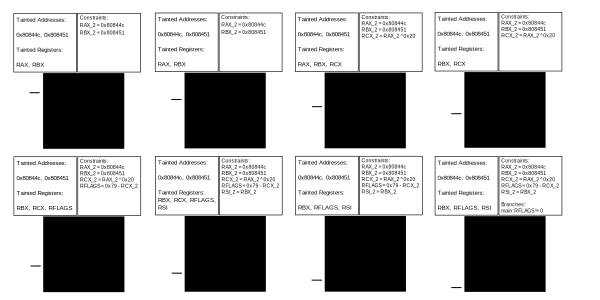
\includegraphics{taintprop}
 \caption{Taint Propogation Example}
 \label{figure:taintprop}
\end{figure}

The basic design of the taint system is that we initially capture any reads from
the file descriptor referencing our ``tainted input''. We can then keep track of
any memory addresses or locations that this ``tainted input'' is stored
in. We also mark each of the original reads from the tainted file with a special
marker that is then used by the Concolic System. Then, we analyze each
instruction in the program and if its a read from a tainted location (memory or
register), we create a new constraint representing the instruction and taint the
resulting location. In this way, as the program executes the set of tainted
registers and addresses slowly changes at each instruction. Finally, we can keep
track of any branches that occur in the program and check whether they are
controlled by the ``tainted input'' by seeing if the values the branch is
depended on is tainted at that time. Figure \ref{figure:taintprop} shows an
example of how this system works.

\begin{figure}[ht]
 \centering
 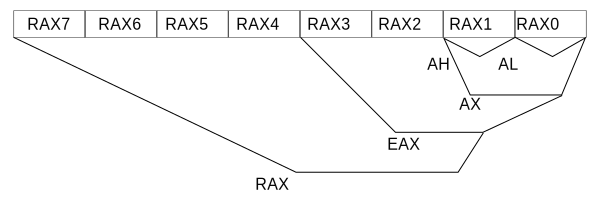
\includegraphics{taintregs}
 \caption{Register Chunks Example}
 \label{figure:taintregs}
\end{figure}

However this design doesn't deal with the fact that we have instructions that
move registers of differing lengths. In order to deal with this, we instead keep
track of each register as chunks of 8 bits. Therefore most registers, which tend
to be 64-bit, are made of 8 chunks numbered $R{\it N}X0$ through $R{\it  N}X7$.  
Depending on the size of the operation that moves data around, we copy
over a certain series of register chunks over, keeping the previous values for
the uncopied registers. Figure \ref{figure:taintregs} shows the layout described
and how the various register chunks are related.

Each tainted operation we encounter then generates the constraints depicted in
Figure \ref{figure:regexample}, which while more than the original design
doesn't add that much complexity for z3 to solve against, since most of the
constraints are under constrained or simple substitutions.

\begin{figure}[t]
\centering
\begin{verbatim}
Tainted: RAX0_1, RAX1_1

Instructions:
  mov bx, 0x2020
  xor ax, bx


Tainted: RAX0_1, RAX1_1, RAX0_2, RAX1_2
Tainted Instructions:
  RAX_AX_2: xor ax, bx ::: 0x2020 + RAX_AX_1 -> RAX_AX_2


New Constraints:
 RAX_AX_1 = {RAX1_1, RAX0_1}

 RAX_AX_2 = OP(RAX_AX_1 + 0x2020)

 RAX1_2 = RAX_AX_2[1]

 RAX0_2 = RAX_AX_2[0]
\end{verbatim}
\caption{Register Constraints Example}
\label{figure:regexample}
\end{figure}

Once the Taint Analysis system has finished generating the list of tainted
instructions and a semantic for how the registers are altered, it produces a
text file listing all the tainted branches that were encountered, along with the
list of tainted instructions/constraints. While the instructions are separated
into separate registers and rough constraints at the taint analysis stage, it
isn't until the generated file enters the Concolic system that the constraints
are parsed and turned into a form more suitable for our constraint solver.

\section{Concolic System Design}
The Concolic System has many components working together to generate new inputs
and to call out to the Taint Analysis system. It first generates an initial
blank input which is sent to the Taint Analysis system. Then, for each input it
has sent off it first parses the response, generating SMT constraints
representing the state of the program and each branching point. Then it proceeds
to attempt to solve the constraints for new inputs that can once again be sent
off to the Taint Analysis system. If we have already observed an input, we skip
it since we've already parsed it, and once we are unable to generate new inputs
that traverse unexplored parts of the program, we conclude the fuzzing. We'll
discuss each of these stages in turn.

\subsection{Taint Analysis Parsing}
This stage turns the Taint Analysis output from something like 
``RFLAGS\_0\_1: cmp al, 0x6c ::: RFLAGS\_0\_1 = OP(RAX\_0\_1, 0x6c)'' into a SMT
equation of the form ``RFLAGS\_0\_1 == 0x6C - RAX\_0\_1''. We don't generate the
actual SMT form until this stage in order to allow the Taint Analysis system to
be disconnected from the format of the SMT system we are using. This stage is
actually split into two parts, one to handle the parsing of the actual branches
that have been encountered and another to parse the general
instructions/constraints that we've picked up throughout the execution of the
program.

For each branch, we also need to figure out whether the branch was taken during
this execution so that the Path Exploration system can determine what branches
haven't been visited. Since almost all branches are based on the state of
RFLAGS, we also have the Taint Analysis provide the concrete values of RFLAGS so
that we can determine whether the path has been taken depending on the opcode of
the branch instruction.

For general instructions/constraints, we parse each instruction to convert the
opcode into an actual operation between the arguments of the instruction. There
are three categories of instructions, those that take a single argument, those
that take two arguments, and finally those that also modify RFLAGS. Using both
the semantics of the arguments and the opcode, we can determine the appropriate
operation to perform between the operations.

Once we've gathered a series of SMT equations representing all the steps of the
program execution, as well as a separate series of equations representing each
of the branches we've taken, we pass this onto the Path Exploration system to
generate subsets of the branch equations for Input Generation.

\subsection{Path Exploration}
Once we've generated the initial SMT equations, we need to start generating the
various different sets of branch paths we want to explore in subsequent
tests. The way we generate each of these new branch paths is by going through
each of the branches we've hit, and keeping all previous branch constraints
while we negate the current branch constraint. Figure \ref{figure:pathexplore}
shows the initial path that we've explored, as well as the additional paths
we'll try exploring in the new inputs. We don't worry about de-duplicating paths
at this point since we'll de-duplicate repeated inputs as part of the input
generation phase.

\begin{figure}[ht]
 \centering
 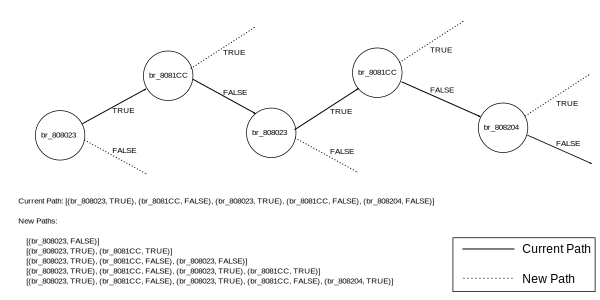
\includegraphics{pathexplore}
 \caption{Path Exploration Example}
 \label{figure:pathexplore}
\end{figure}

Once we've figured out which branch constraints to keep and which to negate, we
can simply add a new constraint of ``AND(branches[:i], NOT(branches[i]))''. Once
we have all the constraints, we send them to the SMT solver to solve and
generate concrete values for all the variables. Once this step is done, the
result can be passed to the Input Generation phase to create new test cases.

\subsection{Input Generation}
Once we've solved the SMT equations to find concrete values for each of the
variables in the constraints, we actually have to generate an input using these
concrete values. While normally straightforward, we have to deal with parts of
the tainted file that may never have been read by the current execution of the
program or other edge cases. Instead what we do is first find the size of the
tainted file that we need to create, by finding the largest value for which a
symbol is defined representing the tainted input file and creating an initial
array representing the file defaulting to using the null byte. Once we've
generated the array, we replace the values that we have concrete values for from
the SMT solver and generate a file.

While using null bytes as the default could have problems since some code stops
parsing a file at the nullbyte, we would have a constraint representing this
case in the list of constraints from the program execution, so we don't need to
add a special exception for that case.

Its at this stage that we deal with de-duplicating inputs that we already have
seen. This prevents us from revisiting paths that we have already
analyzed. Another way with dealing with duplicate inputs is to keep track of the
sets of paths that have been explored and then checking our new path against
that list.

\section{Minor Component Design}
In addition to these major components of \textit{Confuzzer}, we also have a
number of other smaller components that are used to help make the system more
efficient and to allow greater usability.

\subsection{Distributed Nodes}
\begin{figure}[ht]
 \centering
 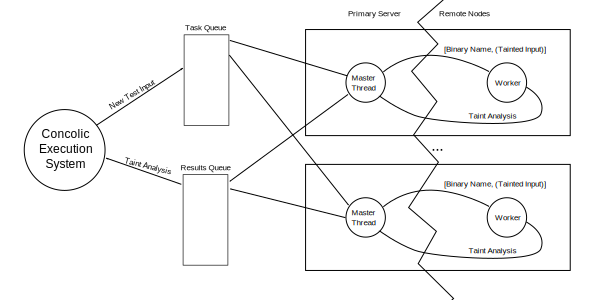
\includegraphics{distnodes}
 \caption{Distibuted Nodes for Taint Analysis}
 \label{figure:distnodes}
\end{figure}

One of the first optimizations made to the design is the ability to distribute
the workload from a single machine to many. We achieve this by creating workers
running on various servers that accept tasks that detail the value that should
be used for the tainted input, as well as the filename to execute. To prevent
malicious use of this system, we require that the binary being tested be
uploaded to the servers through a separate channel. Figure
\ref{figure:distnodes} shows the overall design of the distributed system.

On the worker side, there is a loop while it waits for a task, and once it
receives a task, it creates a new directory with a copy of the binary and all
files accessed by the binary. It then runs the Taint Analysis tool on the binary
in that directory, and upon completion returns the result of the Taint Analysis
to the master. This design is done so that different executions of the binary
don't interfere with each other, and to keep a log of all binary executions on
disk in case further study of a particular testcase might be necessary at a
later time.

Meanwhile, on the master side, there are threads for each worker, that pull a
task off the synchronized queue (filled by the Input Generation phase) and send
them over RPC calls to the various workers. The queue is prioritized based on
metrics from the Concolic Execution system and the Graph Viewer (described
below). Once a worker has completed its task, the results are stored in another
queue to be returned to the Concolic system.

This design allows us to run a lot of tests at the same time without having to
wait for each one to complete. Since the slowest part of the system is the Taint
Analysis system, this distributed system greatly improves the time it takes to
run lots of tests. For larger programs, the Concolic Execution system can also
be distributed across multiple nodes when the SMT solving stage takes a
considerable amount of time.

\subsection{Graph Viewer}
In addition to the other components, we also generate a graph for each new path
that is discovered, and use that to allow a user to prioritize certain branches
when performing further tests.

The graph viewer works by creating a separate node for every branching point and
an edge for both the TRUE and FALSE paths from each branch. Since we are
branching forward from the initial root node, this setup creates a tree
structure that represents all possible branches that we know about so far.

In order to build up the tree, we iterate through each path we've visited and
create a new node for any new branching points and new edges for the direction
that the path travels down. Since the program may sometimes loop back to the
same branching point, we need to keep track of the visited path prefix and
create a new node whenever the new branch happens with a different prefix than
the nodes that we've already drawn, joining paths that have the same prefix and
branch.

Experienced users can use the branching pattern and assembly code disassembly to
select parts of the code to prioritize when generating new paths, allowing the
system to explore all the paths in specific critical sections of the code that
the user might have reason to believe are more vulnerable to malicious inputs.

%TODO: 6 Pages
\chapter{Implementation}
The \textit{Confuzzer} system was implemented with a combination of the Intel
PIN tool to do binary instrumentation and Taint Analysis, and the z3 Python
bindings to actually perform the Concolic Execution step. The current version of
the system is available online at \url{https://github.com/dvorak42/confuzzer}.
The rest of this chapter will discuss the implementation of each of these parts,
as well as the distributed and graphing components.

\section{PIN Taint Analysis Tool}
In order to do the Taint Analysis on the binary, we ended up implementing an
extension for PIN, an Dynamic Binary Instrumenter, to keep track of the tainted
state of memory and registers, and to build up a list of all the instructions
that operated on tainted locations. 

Instead of using a full-system emulator, we ended up choosing to use
an application-specific Dynamic Binary Instrumenter (DBI), since it should have
a lower overhead than emulating an entire system. Of the popular choices, we
ended up using PIN since it was one of the few DBI tools that worked without any
need for compile-time injection and allowed us to fully instrument the program
with easy access to the state of the registers and memory throughout the
program \cite{pintool}. Another option was DynamoRIO, another similar DBI,
however there were fewer systems built on top of it, and had less support at the
time.

The PIN plugin takes in the binary that is being analyzed, as well as the names
of the tainted inputs to the binary. In order to keep track of tainted values,
we first use PIN to instrument any syscalls. Before each syscall, we check the
type of the syscall and if it is an ``open'', we check whether the argument is
one of the tainted files that was passed in, and if so keep track of the file
descriptors referencing these tainted files. Once we have an open tainted file,
we need to check for ``read'' syscalls and label and taint any memory that is
written by the ``read'' syscall.

Once we have a tainted memory location, we need to start instrumenting all
instructions to check whether they are reads from either tainted memory or
registers. Since we need to parse the actual registers and memory locations that
are being affected by the we have different instrumentation functions based on
the number of operands for each operation, and whether they affect registers or
memory locations.

The one special case we need to deal with separately is adding an additional
``branch'' point before predicated instructions. This way, every time that the
predicated instruction, we create a new branch point dependent on the state of
the RFLAG register. The one problem with this approach is that every instruction
will end up instrumented, since we also need to keep track when the taint on
registers and addresses are cleared.

In order to keep track of registers and addresses, we create separate lists for
each. However, since we have instructions that move different size operands, for
each register, we need to separately keep track of each chunk in a
register. While we can do bit-level chunking, x86 primarily affects registers at
a byte level, so the current implementation uses byte-sized chunks. We also
normalize all registers to the largest size ($RDI, RSI, RAX, RBX, \ldots$) when
keeping track of the registers. We also need to keep track of the ID of each
register, so that as we parse new operations that modify the value of the
register, we store it in a newly named variable.

\begin{figure}[ht]
 \centering
\begin{verbatim}
taintRegToReg(instruction, srcReg, dstReg):
  chunkStart, chunkEnd = instruction.offset, instruction.size
  affectReg = []
  for(i in sizeof(dstReg)):
    r1 = {dstReg, i, dstReg.id}
    r2 = {dstReg, i, dstReg.id+1}
    if i < instruction.offset or i > instruction.size + instruction.offset:
      taintEquations.append({'=', r1, r2})

  if isTainted(srcReg):
    s1s = srcReg[chunkStart:chunkEnd]
    s1c = {srcReg, chunkEnd-chunkStart}
    d1s = dstReg[chunkStart:chunkEnd]
    d1c = {dstReg, chunkEnd-chunkStart}
    taintEquations.append({'=', s1s, s1c})
    taintEquations.append({instruction, s1c, d1c})
    taintEquations.append({'=', d1c, d1s})
  else:
    for(i in [chunkStart, chunkEnd]):
      removeTaint(dst)
\end{verbatim}
 \caption{Taint Spread Pseudo-code}
 \label{figure:taintcode}
\end{figure}


Figure \ref{figure:taintcode} shows the pseudocode for actually spreading taint
around the various registers and addresses the program accesses. For any
operations that use tainted registers and addresses, we increment the ID of the
registers being written and then taint them, as well as adding a constraint
representing the assembly instruction. Since we don't want to create constraints
for all registers, we also need to get the value of operands that aren't
tainted. We do this by copying the memory from the source operand, or by using
the Register context that we have to get the current value of an address.

We also need to clear the tainted flag on register and addresses whenever we
have an instruction that moves non-tainted values into a register. Without
clearing the taint flags, we would end up with almost all the registers and
addresses accessed by the program after the original tainted file is read.

Finally we need to keep on propagating any parts of the register that weren't
affected by the current instruction. This is actually a simplification of the
actual code since we need to cast the register chunks together so that the
instruction can operate on them, and then cast it back into separate chunks for
further instructions to interact with.

Whenever we encounter a branching point in the program execution, we check
whether the RFLAGS register is currently tainted, and if so we add the branch to
the list of tainted branches, along with the current value of the RFLAGS
register. This allows us to keep track of which direction each branch was taken
in. While we could keep track of this by checking what the next executed
instruction is, that would require extra bookkeeping.

Separate from the Taint Analysis, we also instrument exception handling in order
to deal with the case of segfaults and other crashes. Since we can't trust that
standard file descriptors for user input and output are still available at this
point, we have to wait until the end of the program's execution to record the
crash/segfault.

At the end of the program's execution, we store all the branching points and
taint constraints in a file for the Concolic Execution System to parse and use
to determine new constraints. In addition, if we recorded a crash or overflow
issue, we also update the execution log with that data. Once we've finished with
the current execution, the Concolic System then takes over to generate new test
cases.

\section{Concolic System}
The Concolic System is implemented using a combination of Python and z3 bindings
to parse the file received from the Taint Analysis system. Every time we receive
the analysis, we parse it in two stages. The first stage parses the taint
constraints into formulas, and the second stage creates the z3 equations.

The first stage parses out the opcode from the assembly instruction and turns it
into symbolic notation. We have to do the parsing in two stages since we need to
build up the set of variables that will be used by the SMT solver. Some of the
assembly opcodes don't have a direct translation to a symbolic equation since we
have a limited set of operations we can use with the SMT solver.

The second stage is where we actually create the z3 variables and the
constraints are actually added to the system. We mark the z3 variables
representing the tainted file inputs differently so that we can later build up
the new input file.

We also have a third stage for our actual branch conditions where we use the
branch opcode and the value of the RFLAGS register at that time to figure out
whether we actually took the TRUE or FALSE path.

Once we've finished parsing all the branches and taint constraints, we can start
iterating through each of them and building up a new path constraint using the
branches we select for this loop and the rest of the taint constraints. Since we
don't have any circular dependencies, and most of the constraints are fairly
straightforward, z3 works fairly well at solving the constraints for satisfiable
sets of constraints, while converging to unsatisfiability for the paths that are
unreachable.

In order to maximize the parts of the program we are exploring early on, we
iterate through each branch on the path and keep the previous branch directions,
while flipping the direction we are exploring on the current branch. So we
create $N$ new paths for every path with $N$ branching points. We then
de-duplicate the repeated paths/inputs once we've converted the solutions from
the SMT solver into actual input files. A good number of paths will end up being
unsatisfiable since there are no inputs to reach that path, or there are
contradictory branches from non-optimized or dead code.

Once we've solved the constraint equations, we generate a new test input and
place it into a test input queue. Its during this phase that we check whether
the input and paths match any of our prioritized branches and if so, we increase
their priorities in the Taint Analysis stage. We keep on parsing outputs and
generating new paths until we work through our queue of inputs and are unable to
generate new unique paths. We also keep track of any paths which result in
crashes/segfaults and mark those as interesting inputs.

\section{Additional Components}
While the previous parts are sufficient to actually run the fuzzer, there are
a few additional components to improve the system. We also have implemented a
distributed system and graph visualization to help with the usability and
efficiency of the system.

We use xmlrpclib and synchronized Queues in order to communicate between the
master and each of the workers. The system is designed to allow each server to
support multiple workers per machine. Each worker can run in separate threads,
listening for the master using different ports. Additionally, each worker thread
can run multiple PIN Taint Analysis processes simultaneously. This allows us to
run about 64 analysis operations at the same time, with 8 threads per machines
on 8 servers.

To prevent security issues with the RPCs being maliciously used, we require that
the binaries that are being used are uploaded to each server through a separate
channel. We also have a script that separately fetches all the log files from
each run through of the taint analysis in order to store any additional
information that the user might want to look over for the crashing test cases.

\begin{figure}[t]
 \centering
 \includegraphics[width=\textwidth]{graphs/1_7}
 \caption{Example Execution Graph}
 \label{figure:samplegraph}
\end{figure}

We use pyplot and graphviz to actually generate the graph of the program
execution. Figure \ref{figure:samplegraph} shows the graph that is generated as
part of the execution of binary. In order to give the user an idea of which
branch each node represents, we also include the assembly instruction that
actually represents the branch.

The user can then input the name of a branch from the graph image into the main
thread in order to prioritize it. Since each node is uniquely identified,
the name of the branch also includes the prefix branches. The user can
prioritize multiple branches in the same part of the program in order to have
the system focus on a specific section of the binary.

While these components don't change the correctness of the system, it does make
the system faster and allow for the user to prioritize parts of the program that
they believe to be vulnerable or critical. There are some additional
optimizations that could be made that will be mentioned in the \textbf{Future
  Work} section in Chapter 6.
\chapter{Evaluation}
To evaluate \textit{Confuzzer}, we compare its performance on our test cases
with the anticipated performance for blind fuzzing and other systems. We can
only calculate expected performance for blind fuzzing, since it would take
longer than available to test some of our test cases.

\begin{table}
\begin{center}
\begin{tabular}{| c | c | c | c | p{6cm} |}
\hline
Test Case & Confuzzer & Blind Fuzzing & AFL & Description\\\hline
test1 & 8 & 1.10e12 & ??? & Simple magic value test\\\hline
test2 & 6 & 1.10e12 & ??? & Keygen test using xored value\\\hline
test4 & 40494 & 1.84e19 & ??? & Toy shell example without overflow\\\hline
test4 & 40494 & 1.84e19 & ??? & Toy shell example with overflow\\\hline
\end{tabular}
\end{center}
\caption{Test Cases per Fuzzing System}
\label{table:evalcases}
\end{table}

\begin{table}
\begin{center}
\begin{tabular}{| c | c | c | c | c | p{6cm} |}
\hline
Test Case & Confuzzer & Confuzzer (Distributed) & Blind Fuzzing & AFL\\\hline
test1 & 0.21 runs/sec & 3.2 runs/sec & 2513 runs/sec & 9850 runs/sec\\\hline
test2 & 0.20 runs/sec & 3.1 runs/sec & 2497 runs/sec & 9879 runs/sec\\\hline
test3 & 0.18 runs/sec & 2.7 runs/sec & 2454 runs/sec & 10.8k runs/sec\\\hline
test4 & 0.17 runs/sec & 2.7 runs/sec & 2434 runs/sec & 11.3k runs/sec\\\hline
\end{tabular}
\end{center}
\caption{Fuzzing Speed}
\label{table:evaltime}
\end{table}

We first look at the number of test cases that our fuzzers generate, since
programs of similar complexity will have roughly the same branching amounts,
giving us a better picture of how each system scales. Our rough results are in
Figure \ref{table:evalcases}. The estimate for blind fuzzing is based on the
number of possible inputs before we are likely to hit a crashing input. We
weren't able to make measurements for AFL, since it wasn't able to determine
sufficient information to prioritize certain kinds of input, even with a basic
set of example inputs for the test application. One of the advantages of AFL is
that it is able to notify the user of crashing inputs while still running,
compared to the current implementation of Confuzzer.

We then measure the amount of time each fuzzing system takes to run test cases,
to show how the speed of the Confuzzer compares to the other systems. Figure
\ref{table:evaltime} shows that the speed of the Confuzzer system is orders of
magnitudes slower than the other systems. We actually end up having better
timing from AFL than Blind Fuzzing since it forks the binary instead of creating
a new process for every test case.

This shows how the Concolic Fuzzer system is able to hone in on specific
interesting inputs without having to hit a ton of unnecessary inputs, however
the process of finding inputs takes a long time and is heavily dependent on the
size of paths in the binary being fuzzed.

While the test cases we are using for the system are a bit artificial, there are
many existing programs that have similar constructs, including parsers that
search for magic values in order to figure out whether a file is valid, key
verification systems that check whether an input is valid to detect some key
file is valid, and even network protocols that expect a certain class of inputs.

From the timing results, we could probably end up with a more efficient system
by using a combination of \textit{Confuzzer} to generate inputs that pass
through taint checks, and then using AFL or another Fuzzer in order to look for
alternate inputs past the initial checks in the program. Unfortunately doing
this sort of merged Fuzzing requires either some amount of user input to
determine when to switch between the systems, or some sort of heuristic to deal
with moving between the fuzzers.

The results for AFL also show that its possible that moving from a PIN
instrumenter to something using QEMU User Mode Emulation might offer an
improvement in the running time of the system. Most of the slowness in running
the Confuzzer system comes from the context switching and instrumentation of the
binary code. We can increase the speed of the Fuzzer using our distributed
system to run multiple instances of the binary and Taint Analysis system. Some
of the additional improvements we can apply to \textit{Confuzzer} are covered in
the \textbf{Future Work} section in Chapter 6.

% TODO: 2/4 Pages
\chapter{Future Work}
While we currently have a working system, there is still a lot of work that can
be done to improve the overall system and create a more efficient and useful
system. Similar to the Design, we can split this into two major categories of
work, work for the Taint system and work for the Concolic Execution system.

\section{Taint Analysis Improvements}
One of the major improvements to the Taint Analysis system is to switch from
using Intel PIN to another instrumentation tool. Some options to explore, given
other Taint Analysis and fuzzing tools are using DynamoRIO as its support
improves, using full-system emulation, and finally using QEMU's user mode
emulation. The final option seems to be most likely to give improved results,
given the success that AFL has had with it.

In addition to switching the Taint Analysis to a different system, we can also
reduce the set of instructions that we have to examine by detecting standard
functions that we trust and instead of instrumenting the function execution, we
add special constraint equations to the Taint log. One example is being able to
detect strcmp and other related functions, and replacing them with constraints
that represent the possible return values from the functions, rather than having
tons of branching points and constraints within the library function
itself. There are a couple ways of doing this, from using some huerestic to
detect known functions, or actually stubbing out the real library we are
optimizing with one that has markers that the Taint Analysis tool would be able
to detect and choose to pause instrumentation.

Another improvement that needs to be made to the Taint Analysis system is
support for additional types of tainted input, either more general user input
from the console, to actual data packets through network sockets. Having these
additional forms of tainted input would allow us to test more parts of the code
without having to have artificial wrappers that convert a file input into a
network or user input.

Finally, the last major improvement to the Taint Analysis system that would be
useful is the addition of more ways to detect ``bad'' or potentially troublesome
states, some can be as simple as invalid memory access detection (which already
can be done with PIN) or even so far as detecting unintentional control flow
hijacking or policy violation. These would allow the system to detect a wider
array of potential issues all at once.

\section{Concolic Execution Improvements}
On the Concolic Execution end, one improvement is to the way we handle
constraints. If we are able to reduce the number of variables we create when
parsing the tainted assembly instructions, we could reduce some of the work z3
has to do when solving the equations. Similarly, if we are able to detect more
compound data structures, such as strings, we would be able to combine many of
the generated constraints together and use things like z3str for string
computations.

Additionally, if we were able to do better path and loop detection, we could
improve the search algorithm we use to search more interesting parts of the
program space without spending a bunch of time repeatedly working on the same
looping structure. Generally, having an improved search algorithm and
prioritization would allow us to reach interesting test cases much earlier.

Another overall improvement to the system that should be done in the future is
adapting it to work together with other existing Fuzzers. While
\textit{Confuzzer} has a advantage on some test cases that other fuzzers have
trouble with, the existing fuzzers also have their own advantages on other parts
of the program execution. Allowing multiple fuzzers to work together would allow
a wider search of the program input space without having all the test cases take
as long as the \textit{Confuzzer} test cases take.
\chapter{Conclusion}
In this thesis, we presented \textit{Confuzzer}, an implementation of a Concolic
Execution Fuzzer to help with finding inputs to the program that can cause
malicious behavior. Unlike most existing Fuzzers, Concolic Execution allows us
to get through sections of the binary that require matching certain values and
allowing us to get past sections that would otherwise cause other Fuzzers to
take a long amount of time. In implementing this system, we've aimed to design
the system to allow the analysis of as many binaries as possible, without
requiring source code to perform the analysis. While this prevents us from
constructing Intermediate Representations to use in doing the taint analysis, we
are still able to parse x86 instructions sufficiently to determine how to spread
taint through the program.

While there are still many improvements that could make to the system, the
initial prototype is already able to test a class of programs that are difficult
to test with the existing systems. Being able to programatically generate test
cases is an important step in better securing existing code and doing in-depth
testing fast enough to be effective against determined attackers.

\appendix
\chapter{Example Program}
In order to demonstrate the success of the \textit{Confuzzer} system, we've
included the code for a simple test application as well as excerpts from its
execution under the Confuzzer system. Using a single execution node, this test
took about 14 hours and generated a total of around 40500 unique inputs, without
pruning, to the program. 

\lstinputlisting[language=C++]{test4.c}

This program works by taking in 8 instructions as part of a text file, each of
which could either ``[l]ist'' the files that have been created, ``[w]rite'' a
new file, or ``[d]ump'' the contents of the files. Due to an implementation bug,
this code has a memory corruption error if too many files are written. Since
this was compiled on a 64-bit system, this tends to occur when more than 4 files
are written to memory. Below is a part of the output from the fuzzer, showing
the test cases that were sent to the Taint Analyzer, as well as the newly
generated test cases from each execution:

\begin{multicols}{2}
\begin{verbatim}
Testing ./test4 with:
 Tainted input 'script.txt'
Left: 1
1 l
1 w
1 d
1 t
1 $l
1 $w
1 $d
1 $�
1 $_l
1 $_w
1 _�
1 $_d
Left: 12
2 
Left: 12
3 wl
3 ww
3 wd
3 wt
3 w$l
3 w$w
3 w$d
3 w$�
3 w$_l
3 w$_w
3 w$_d
3 w$_t
3 w$__l
3 w$__w
3 w$__d
3 w$_c�
3 w$�__l
3 w$�__w
3 w$�__d
3 w$P�C�
3 w$O_?_l
3 w$O_?_w
3 w$O_?_d
3 w$__c`�
3 w$_____l
3 w$_____w
3 w$_____d
3 w$___�?_
Left: 39
4 �
Left: 39
5 $_t
5 $__l
5 $__w
5 $__d
5 $_c�
5 $�__l
5 $�__w
5 $�__d
5 $P�C�
5 $O_?_l
5 $O_?_w
5 $O_?_d
5 $__c`�
5 $_____l
5 $_____w
5 $_____d
5 $_X_c_�
5 $___�?_l
5 $___�?_w
5 $___�?_d
5 $`______
Left: 59
...
Left: 5
Left: 4
Left: 3
Left: 2
Left: 1
40481 wwwwwwl
40481 wwwwwww
40481 wwwwwwd
40481 wwwwwwt
40481 wwwwww$l
40481 wwwwww$w
40481 wwwwww$d
40481 wwwwww$_
Left: 8
40482 wwwwwwll
40482 wwwwwwlw
40482 wwwwwwld
40482 wwwwwwl$
Left: 11
Left: 10
Left: 9
Left: 8
40486 wwwwww$l
40486 wwwwww`
Left: 9
Left: 8
40488 wwwwwwd
Left: 8
Left: 7
Left: 6
Left: 5
40492 wwwwwwl^D
Left: 5
Left: 4
40494 wwwwwwl$
Left: 4
Left: 3
Left: 2
Left: 1
\end{verbatim}
\end{multicols}

A subset of the crashing inputs that were discovered is below:

\begin{verbatim}
Crashing Inputs:
        $_wwwwdw
        $_wwwwlw
        $wdwwwdw
        $wdwwwwl
        $wldwwww
        $wlw_www
        $wlwdwww
        $wlww_ww
        $wlwwww
...
\end{verbatim}

This along with the remaining crashing inputs covers most of the space of inputs
that should crash the program, showing that even with a program that has a
combinatorial explosion of paths $4^8$, Confuzzer is still able to function in a
reasonable amount of time. The 14 hours for $~40000$ paths matches closely with
the results observed by the SAGE system \cite{sage}. With the use of N nodes,
the time needed to run this test could be reduced by about a factor of $N$,
since the majority of the time was spent in the actual execution of the programs
with different inputs.
\chapter{Example Execution Graphs}
Attached is the code and execution graphs for some of the simpler test cases
we've been using.

\lstinputlisting[language=C++,basicstyle=\tiny,caption=test1 Source Code]{test1.c}

\lstinputlisting[language=C++,basicstyle=\tiny,caption=test2 Source Code]{test2.c}

\begin{figure}[ht]
 \centering
 \begin{tabular}{| c | c |}
   \hline
   \includegraphics[width=0.45\textwidth]{graphs/1_0}
   &\includegraphics[width=0.45\textwidth]{graphs/1_1}\\\hline
   \includegraphics[width=0.45\textwidth]{graphs/1_2}
   &\includegraphics[width=0.45\textwidth]{graphs/1_3}\\\hline
   \includegraphics[width=0.45\textwidth]{graphs/1_4}
   &\includegraphics[width=0.45\textwidth]{graphs/1_5}\\\hline
   \includegraphics[width=0.45\textwidth]{graphs/1_6}
   &\includegraphics[width=0.45\textwidth]{graphs/1_7}\\\hline
 \end{tabular}
 \caption{Example Execution Graphs for test1}
 \label{figure:examplegraphs}
\end{figure}

\begin{figure}[ht]
 \centering
 \begin{tabular}{| c | c |}
   \hline
   \includegraphics[width=0.45\textwidth]{graphs/2_0}
   &\includegraphics[width=0.45\textwidth]{graphs/2_1}\\\hline
   \includegraphics[width=0.45\textwidth]{graphs/2_2}
   &\includegraphics[width=0.45\textwidth]{graphs/2_3}\\\hline
   \includegraphics[width=0.45\textwidth]{graphs/2_4}
   &\includegraphics[width=0.45\textwidth]{graphs/2_5}\\\hline
   \includegraphics[width=0.45\textwidth]{graphs/2_6}
   &\includegraphics[width=0.45\textwidth]{graphs/2_7}\\\hline
 \end{tabular}
 \caption{Example Execution Graphs for test2}
 \label{figure:examplegraphs2}
\end{figure}

\include{biblio}
\end{document}

